\chapter{Mechanik des starren K"orpers}
\label{kap_mechanik-des-starren-korpers-1}


Wir betrachten nun starre, ausgedehnte K"orper. Anders als bei
Massenpunkten sind die Abst"ande zwischen den einzelnen Teilchen nun
fest -- die betrachteten K"orper sind nicht deformierbar (deswegen
hei"sen sie \emph{starr}).

Als "`Ersatz"' f"ur einzelne Massenpunkte $m_i$ k"onnen wir hier
verwenden:
\begin{equation}
   \label{eq:33}
   \diff m (\vec r) = \varrho (\vec r) \cdot \diff V
\end{equation}
wobei $\varrho(\vec r)$ die \emph{Dichte} des Stoffes am Ort $\vec r$
ist.









\section{Statik}
\label{kap_statik}


Hier wollen wir die Bedingungen untersuchen, unter denen sich ein
K"orper \emph{nicht} bewegt:

Anschaulich ist sofort klar:
\begin{Wichtig}
   [1. Bedingung f"ur mechanisches Gleichgewicht]
Die Summe der angreifenden Kr"afte muss verschwinden.
\begin{equation}
   \label{eqn_statik_bed_kraft}
   \boxed{
\sum_i \vec F_i = \vec 0
}
\end{equation}
\end{Wichtig}

In Abb. \ref{abb_wippe} ist dagegen eine Wippe abgebildet. Auch wenn
$F_1 + F_2 + F_c = 0$, so wird die Wippe dennoch kippen  -- ebenfalls
anschaulich klar.

Wir wir im Vorangegangenen Kapitel gesehen haben, wird auf die Wippe
so n"amlich ein \emph{Drehmoment} ausge"ubt, wodurch sich ein
\emph{Drehimpuls} ergibt, welcher f"ur das Kippen verantwortlich
ist.\footnote{Das Drehmoment von $F_e$ verschwindet, weil hier $\ell =
  r=
  0$. Au"serdem d"urfen wir ohne Kreuzprodukt rechnen, weil $r \bot F$
  und wir praktisch an den Betr"agen interessiert sind, \emph{weil wir
    die Richtung des Drehmoments wissen}.}
\begin{equation}
   \label{eq:36}
   \ell_1 \cdot F_1 + \ell_2 \cdot F_2 \neq 0 ~ \Rightarrow ~ L \neq const
\end{equation}
Damit wir $M_{ges} = 0$ bekommen, m"ussen wir {ersatzweise} die Kr"afte $F_2'$ und
$F_e'$ angreifen lassen. Dann gilt n"amlich:
\begin{Wichtig}
   [2. Bedingung f"ur mechanisches Gleichgewicht]
Die Summe der angreifenden Drehmomente muss verschwinden.
\begin{equation}
   \label{eqn_statik_bed_drehmoment}
   \boxed{
\sum_i \vec M_i = \vec 0
}
\end{equation}
\end{Wichtig}

\begin{figure}
   \centering
   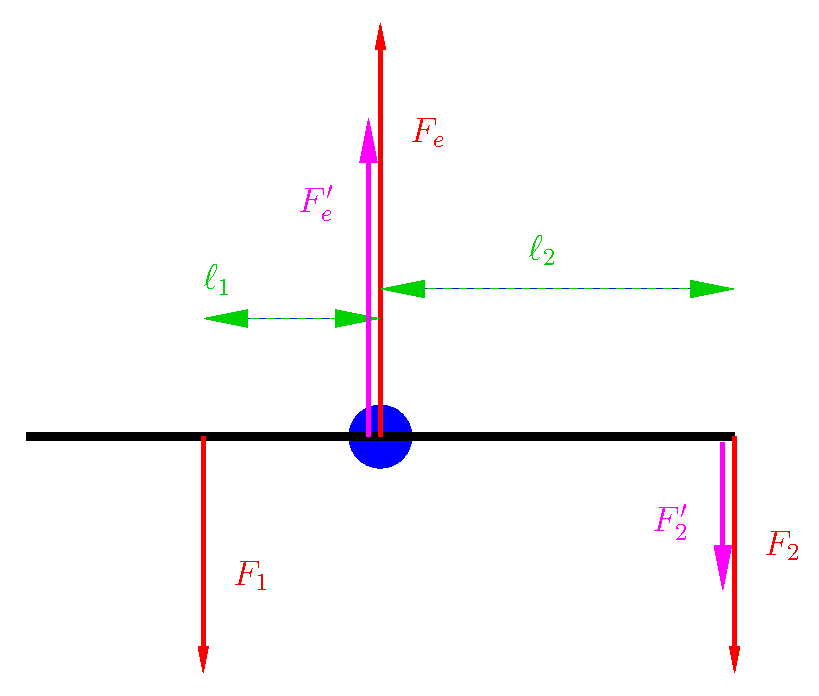
\includegraphics[width=0.7\textwidth]{bilder/wippe}
   \caption[Wippe im Gleichgewicht]{Wippe auf die Kr"afte wirken. Die
     Kr"afte $F_e'$ und $F_e$ sowie $F_2'$ und $F_2$ sollen \emph{am
       gleichen Punkt} angreifen.}
   \label{abb_wippe}
\end{figure}

\bigskip

Daraus folgen auch direkt die
\textbf{\index{Hebelgesetze}Hebelgesetze}: Damit der
Drehimpulserhaltungssatz gilt, muss
\begin{equation}
   \label{eqn_def_hebelgesetz}
   \boxed{
F_1 \cdot \ell_1 = F_2' \cdot \ell_2
}
\end{equation}
dabei werden die $\ell$ vom Hebelpunkt aus gemessen und die Kr"afte $F$
senkrecht zu $\ell$.

\bigskip

\subsubsection{verschiedene Arten von Gleichgewichten}
\begin{description}[\setlabelstyle{\bfseries\slshape}]
\item[Stabiles] Auf"angung "uber Schwerpunkt $S$\\Bei der Auslenkung wird
   $S$ angehoben und $E_{pot}$  steigt. Der K"orper wird sich also
   nicht von selbst auslenken, sondern in der Ruheposition -- auch bei
   kleinen St"orungen -- verharren.
\item[indifferentes] Die Aufh"angung liegt direkt auf dem Schwerpunkt
   $S$\\Bei Bewegung (Drehung) "andert sich weder $S$ noch
   $E_{pot}$. F"ur diese Aufh"angung sind (unendlich) viele verschiedene
   Orientierungen m"oglich.
\item[labil] die Aufh"angung liegt unter dem Schwerpunkt $S$\\Schon bei
   einer minimalen Auslenkung "`kippt"' das System und
   f"uhrt\footnote{bei Reibung -- hier schwingt es ged"ampft und kommt
     irgendwann zur Ruhe; ohne Reibung wird die Schwingung ewig gehen.} zu einer neuen Gleichgewichtslage.
\end{description}


\subsubsection{Standfestigkeit eines K"orpers}
\label{kap_standfestigkeit-korpers}

\begin{figure}
   \centering
\includegraphics[width=0.7\textwidth]{bilder/schwerpunkt}
   \caption[Vergleich: Stabil, instabil]{Drei K"orper (vlnr): stabil,
     labil, wird gleich kippen}
   \label{abb_standfestigkeit}
\end{figure}

Falls die Projektion des Schwerpunkts $S$ auf die Grundfl"ache
au"serhalb der Standfl"ache selbst liegt, so wird der K"orper kippen.
Er dreht sich dann "uber seinen
\textbf{Drehpunkt}. (Vgl. Abb. \ref{abb_standfestigkeit}) Wenn der
Schwerpunkt wirklich "uber der Grundfl"ache ist, so m"usste der K"orper,
um zu kippen, seinen Schwerpunkt zuerst anheben und daf"ur br"auchte er
Energie. In Abb. \ref{abb_standfestigkeit} wird also nur der rechte
K"orper von selbst kippen -- hier kann der K"orperschwerpunkt bequem
(nur) nach unten fallen.




\section{Dynamik}
\label{kap_dynamik}

Wir unterscheiden zwischen \textbf{zwei Arten von Bewegung}:
\begin{description}[\setlabelstyle{\bfseries\slshape}]
\item[\index{Translation}Translation] Die Masse wird einfach
   verschoben. F"ur jeden einzelnen Massenpunkt gilt die gleiche
   Verschiebung: $\forall_i: \vec r_i \mapsto \vec{r_i}' = \vec r_i +
   \vec c(t)$. Dabei kann $\vec c$ nat"urlich von der Zeit abh"angen.

   Wir k"onnen uns dabei die gesamte Masse $M$ im Schwerpunkt des
   K"orpers konzentriert vorstellen.
\item[\index{Rotation}Rotation] Die einzelnen Massenpunkte werden
   abh"angig davon, wie weit sie vom Rotationszentrum entfernt sind,
   verschoben: $\forall_i: \vec r_i \mapsto \vec{r_i}' = \Mat{R} \cdot
   \vec r_i$. Dabei kann die Rotationsmatrix $\Mat{R} \in SO(3)$ von
   Zeit und Ort abh"angen.

Alternativ kann man eine Rotation auch mit $\vec \omega$ darstellen:
Der Drehvektor $\vec \omega$ laufe durch den Schwerpunkt $S$ des
K"orpers. Wir verwenden als Relativkoordinaten ein System mit $S$ als
Ursprung: $\vec r_{Si}$ beschreibt den Vektor zwischen $S$ und dem
$i$-ten Massenelement ($\vec r_{Si} = \vec r_i - \vec r_S$). Dann ist
die Rotationsgeschwindigkeit f"ur dieses Element gegeben durch
\begin{equation}
   \label{eqn_rotationsgeschwindigkeit}
   \vec v_r = \vec \omega \times \vec r_{Si}
\end{equation}
Dabei kann $\vec \omega$ nat"urlich wieder abh"angig von Ort und Zeit
sein.\footnote{Hier kann man sch"on die \emph{Rechte-Hand}-Regel
  anwenden: Rotiert ein K"orper, bildet der Daumen die Rotationsachse
  nach und die Finger der Faust zeigen in die Richtung der
  Drehung. W"ahlt man nun einen Vektor $\vec r$ so stellt man diesen
  mit dem Zeigefinger dar und erh"alt aus dem Mittelfinger die Richtung
  der Geschwindigkeit.}
\end{description}


\begin{Wichtig}
   Sobald eine Kraft an einem Punkt verschieden vom Schwerpunkt
   angreift, sorgt sie daf"ur, dass der K"orper rotiert.
\end{Wichtig}





\subsection{Drehimpuls eines starren K"orpers}
\label{kap_drehimpuls-starren-korpers}


Um den Drehimpuls eines K"orpers zu berechnen, m"ussen wir seine Form
und seine Massenverteilung einbeziehen. Wir zerlegen ihn im Allgemeinen
in unendlich viele kleine Massenelemente, deren Drehmomente wir
einzeln berechnen und schlie"slich aufaddieren:
\begin{equation}
   \label{eq:39}
   \vec L = \sum_i m_i \cdot (\vec r_i \times \vec v_i) = \sum_i \vec L_i
\end{equation}
Dabei gehen wir zum Grenzwert "uber und erhalten statt der Summe $\sum_i$
ein Integral $\int_V$.

Verwenden wir nun $\vec v_i = \vec \omega \times \vec r_i$, kommen wir
nach Gl. \eqref{eqn_drehimpuls-in-kreis} auf $\vec L_i = m_i \cdot
r_{\bot, i}^2 \cdot \vec \omega$. (Da der \emph{ganze} K"orper mit $\vec
\omega$ rotiert, ist das $\vec \omega$ an allen Stellen des K"orpers
gleich.)  Das $r_{\bot, i}$ bezeichnet den (senkrechten) Abstand von
$m_i$ zur Drehachse.  Verwenden wir nun anstelle der diskreten Massen
$m_i$ die Massenverteilung $\varrho(\vec r)$ (also $\diff m = \varrho
(\vec r) \diff V$), so erhalten wir aus Gl. \eqref{eq:39}:
\begin{equation}
   \label{eq:40}
   \vec L = \left ( \underbrace{\int_V \varrho(\vec r) \cdot  r_\bot^2 \diff V}_I
     \right ) \cdot \vec \omega
\end{equation}

\subsection{Tr"agheitsmoment}
\label{kap_tragheitsmoment}



\begin{Def}
   [\index{Tr"agheitsmoment}Tr"agheitsmoment]
\label{def_traegheitsmoment}
Das Tr"agheitsmoment 
\begin{equation}
   \label{eqn_def_traegheitsmoment}
   \boxed{
I = \int_V \varrho(\vec r) \cdot \vec r_\bot^2 \diff V
}
\end{equation}
"ubernimmt bei einer Drehbewegung die Rolle der Masse bei einer
geradlinigen Bewegung\footnote{Vgl. $\vec p = m \cdot \vec v$}. Hier
ist $\vec r_\bot$ senkrecht zu $\vec\omega$. Es gilt
\begin{equation}
   \label{eqn_drehimpuls-aus-traegheit}
   \vec L = I \cdot \vec \omega
\end{equation}
\end{Def}


Dabei muss $I$ jedoch kein Skalar sein -- $I$ ist vielmehr ein
\textbf{Tensor} $\Ten I$ (der zweiten Stufe\footnote{Geh"ort zu einer
  Linearen Abb. $R^n \to R^n$ -- hier $n = 3$.}). Das liegt daran, dass der
K"orper in verschiedene
Richtungen unterschiedlich einfach rotierbar ist.
Bspw. kann man einen Zylinder in einer Raumrichtung ohne
Energieaufwand rotieren (um ihre \emph{Rotations}achse) und in die
anderen nur schwer.

Der Tensor $\Ten I$ ist gegeben durch
\begin{equation}
   \label{eqn_traegheitstensor}
   \Ten I = I_{ij} = I_{ji} = \int_V \varrho(\vec r) \cdot (
   \delta_{ij}\vec r^2 - r^i \cdot r^j ) \diff V
\end{equation}
d.h. der Tensor ist \emph{symmetrisch}. Dabei stehen die Indizes $i$
und $j$ f"ur die $i$-te bzw. $j$-te Komponente des $\vec r$ im
Kartesischen Koordinaten (also ist bspw. $r^1 = x$). Entsprechend
hei"sen die einzelnen Elemente von $\Ten I$ auch $I_{xx}$, $ I_{xz}$, usw.

Um mit dem Tensor sinnvoll zu rechnen, kann man aus ihm das
\emph{Tr"agheitsmoment} $I_A$ bez"uglich einer Achse $A$ errechnen. Dazu
bildet man den Normalenvektor $\vec e_A$ parallel der Geraden mit
$\|\vec e_A\| = 1$ und multipliziert $\Ten I$ damit:
\begin{equation}
   \label{eq:44}
   I_A = {\vec e_A}^{T} \cdot  \Ten I \cdot \vec e_A
\end{equation}

\abs
Betrachten wir den Tensor als \emph{Matrix}, so wissen wir, dass man
jede symmetrische Matrix \emph{diagonalisieren} kann. D.h. wir k"onnen
eine \textbf{Hauptachsentransformation} durchf"uhren, bei der wir unser
Koordinatensystem so w"ahlen, dass unser "`neuer"' Tr"agheitstensor nur
noch auf der Diagonalen Eintr"age hat.

Unsere neu gew"ahlten Koordinaten haben ihren Ursprung im Schwerpunkt
und stehen senkrecht aufeinander. Wir bezeichnen sie als 
\begin{Def}
   [\index{Haupt(tr"agheits)achsen}Haupt(tr"agheits)achsen]
F"ur Rotationen um die Hauptachsen ($\vec \omega_a$, $\vec \omega_b$,
$\vec \omega_c$) ist das Tr"agheitsmoment ein Skalar
-- es ist also 
$$\vec L  ~ \| ~ \vec \omega$$
\end{Def}

Aus der Symmetrie\footnote{Die Symmetrie selbst folgt (auch) aus der Anzahl
  zur Verf"ugung stehender Freiheitsgrade: Eine Rotation im Raum ist
  durch  6 Freiheitsgrade festgelegt (Drei Winkel und drei
  Raumkoordinaten f"ur den Ursprung der Rotation). In unserer $(3 \times
  3)$-"'Matrix"' $\Ten I$ sind also nicht alle Eintr"age frei bestimmbar.} von
$\Ten I$ folgt, dass jeder K"orper \emph{drei} solcher
\emph{Hauptachsen} besitzt. Wie oben gezeigt, kann man jeder davon ein
Tr"agheitsmoment zuordnen. F"ur diese gilt logischerweise:
$$
I_a \leq I_b \leq I_c
$$
Diese bezeichnen wir auch als \textbf{ausgezeichnete} oder
\textbf{Haupt-Tr"agheitsmomente}. F"ur verschiedene Konstellationen
hei"sen die zugeh"origen K"orper\footnote{die "`$\neq$"' und "`$=$"'
  gelten oBdA}:
\begin{center}
\begin{tabular}{l l}
   $I_a = I_b = I_c$ & sph"arischer Kreisel \\
   $I_a \neq I_b = I_c$ & symmetrischer Kreisel \\
   $I_a \neq I_b \neq I_c$ & asymmetrischer Kreisel 
\end{tabular}
\end{center}


\subsubsection{Freie Achsen $(\bigstar)$}
\label{kap_freie-achsen}

Versetzt man einen K"orper in freie Rotation -- also h"alt keine
Rotationsachse k"unstlich fest -- so rotiert er nicht unbedingt einfach
weiter, sondern beginnt zu \emph{eiern}: 

$$
\vec L \not \parallel \vec \omega
$$

Bei folgenden (Sonder)F"allen eiern die K"orper \emph{nicht}, sonder
rotiert so, als w"are es eine feste Achse:
\begin{itemize}
\item Der K"orper rotiert nur um eine \textbf{Haupttr"agheitsachse}
\item Beim \textbf{sph"arischen} Kreisel
\item Beim \textbf{symmetrischen} Kreisel, der um eine Achse durch den
   Schwerpunkt und senkrecht zur Symmetrieachse rotiert. 
%Sicher: Demtroeder 1, S. 152.
\end{itemize}

\begin{Def}
   [\index{Freie Achsen}Freie Achsen]
sind die Achsen, um die ein K"orper ohne zu eiern rotieren kann, ohne dass man die Achsen festhalten muss.
\end{Def}

\begin{Wichtig}
   Experimentell ergibt sich, dass ein K"orper nur um die Achse seines
   miminalen $\vec I_a$ oder maximalen $\vec I_c$
   Haupttr"agheitsmoments \emph{stabil} rotieren kann.
\end{Wichtig}
Wenn er um die Achse $\vec \omega_b$ rotiert, so reicht schon die
kleineste St"orung aus, dass er zu torkeln beginnt.\footnote{Sch"ones
  Experiment: Ein Quader mit drei verschieden langen Seiten wird
  hochgeworfen und dabei um seine drei Symmetrieachsen rotiert. Bei
  einer der Achsen wirft man ihn hoch und f"angt ihn "`gespiegelt"'
  wieder -- er hat sich im Flug nicht nur um eine Achse gedreht.}




% Betrachten wir einen K"orper, der mit Drehgeschwindigkeit $\omega$ um
% eine bestimmte Drehachse $A$ rotiert ($\vec \omega \| A$), so k"onnen
% wir den Gesamtdrehimpuls  $\vec L$ berechnen, indem wir unseren
% Koordinatenursprung und eine Achse auf $A$ legen und jeden
% Ortsvektor $\vec r_i$ zerlegen in eine Komponente $\vec r_{i\|} \|
% A$ und eine Komponente $\vec r_{i\bot} \bot A$.

% F"ur den Drehimpuls sind nun nur die Vektoren $\vec r_{i\bot}$ wichtig,
% weil nur die \emph{Entfernung} des Massenteilchens von der Achse
% entscheidend f"ur den Drehimpuls ist.



\subsection{Kinetische Energie}
\label{kap_kinetische-energie}



M"ochten wir die \textbf{kinetische Energie} berechnen, die ein K"orper
bei seiner Rotation um eine Achse $A$ mit Rotationsvektor $\vec
\omega$ hat, so integrieren wir "uber die Kinetischen Energien seiner
Massenteilchen:
\begin{equation}
   \label{eq:41}
   E_{rot} = \sum_i \frac{1}{2}m_i v_i^2 = 
\sum_i \frac{1}{2} m_i (r_i \omega)^2 \to 
\int_V \frac{1}{2}\omega^2 m_ir_i^2 =
\frac{1}{2} \omega^2 \underbrace{\int_V r^2 \varrho \diff V}_I
\end{equation}

\begin{Wichtig}
   [Kinetische Energie einer Rotation]
Es gilt
\begin{equation}
   \label{eq:42}
   \boxed{
E_{rot} = \frac{1}{2} \cdot I \cdot \vec \omega^2
} = ~ ~  \frac{1}{2} \cdot \vec \omega^T \cdot \Ten I \cdot \vec \omega
\end{equation}
\end{Wichtig}
Die zweite Form wird verwendet, wenn das Tr"agheitsmoment als Tensor
$\Ten I$ vorliegt.

Vergleiche dazu auch 
$$
E_{kin} = \frac{1}{2} \cdot m \cdot \vec v^2
$$
d.h. wie in Def. \ref{def_traegheitsmoment} angesprochen "ubernimmt $I$
hier wieder die Rolle einer Masse.











\subsection{Drehimpuls verschiedener K"orper}
\label{kap_drehimpuls-verschiedener-korper}



\subsubsection{Rotationssymmetrischer K"orper}
\label{kap_rotationssymmetrischer-korper}

Zu jedem Massenelement $m_i$ geh"ort ein Element $m_i'$. Diese haben zu
$\vec L_{ges}$ die Beitr"age
\begin{eqnarray}
   \label{eq:43}
   \vec L_i &=& m_i \cdot (\vec r_i \times \vec v_i)\\
\nonumber
   \vec L_i' &=& m_i' \cdot (\vec r_i' \times \vec v_i')
\end{eqnarray}
Da der K"orper rotationssymmetrisch ist (Siehe dazu Abb. \ref{abb_rotsym}), ist
$m_i = m_i'$ und $\vec v_i
= - \vec v_i'$. Die Verbindung $\vec r_i - \vec r_i'$ verl"auft
\emph{senkrecht} zur zur Rotation $\vec \omega$. Wir verwenden
$\vec r_{i\bot} = \frac{\vec v_i
 - \vec v_i'}{2}$ (der senkrecht auf der Drehachse steht und zu $m_i$
bzuw. $m_i'$ zeigt), weil uns schlie"slich nur der Abstand von dem
Massenteilchen zur Rotationsachse interessiert.

Ein kleiner Beweis daf"ur\footnote{Aus "Ubersichtlichkeit wurden die
  Indizes gespart.}: Wir zerlegen den Vektor $\vec r$: $\vec r = \vec
r_\bot + \vec r_\|$, wobei $\vec r_\|$ parallel und $\vec r_\bot$
senkrecht zur Drehachse ist. Wegen $\dot{\vec r} = \vec \omega \times
\vec r$ ist 
$$
\vec L = m \vec r \times \vec v = m \vec r \times (\vec
\omega \times \vec r) = m (\vec r_\bot + \vec r_\|) \times (\vec
\omega \times (\vec r_\bot + \vec r_\|))
$$
Mit der Distributivit"at des Kreuzproduktes verschwinden "`hinten"'
Terme mit $\vec r_\|$, weil das Kreuzprodukt paralleler Vektoren
verschwindet:
$$
\vec L = m (\vec r_\bot + \vec r_\|) \times (\vec \omega \times \vec
r_\bot)
=
 m \vec r_\bot \times (\vec \omega \times \vec r_\bot)
+
 m  \vec r_\| \times (\vec \omega \times \vec r_\bot)
$$
Hierauf wendet man BAC-CAP an, und erh"alt:
\begin{equation}
   \label{eq:428}
\vec L = m\vec \omega (r_\bot^2) + m\vec r_\bot (\vec r_\bot \vec
\omega) + m\vec\omega(\vec r_\| \vec r_\bot) - m\vec r_\bot(\vec r_\| \vec \omega)   
\end{equation}
wobei die beiden mittleren Terme trivialerweise verschwinden, weil es
sich um Skalarprodukte orthogonaler Vektoren handelt. Man sieht:
\begin{Wichtig}
   Der Drehimpuls eines einzelnen rotierenden Massenpunktes ist nicht
   parallel zu $\vec \omega$ und ist zeitlich nicht konstant! Nur
   seine Komponente parallel zu $\vec \omega$ bleibt erhalten.
\end{Wichtig}
Weil wir aber f"ur jede Masse $m_i$ noch eine Masse $m_i'$ haben, die
gegen"uber rotiert, gilt f"ur diese $\vec r_\bot' = - \vec
r_\bot$. Addiert man die beiden Drehimpulse $\vec L_i$ und $\vec L_i'$
so f"allt auch der letzte Term aus \eqref{eq:428} weg und $\vec L$ ist
nur noch abh"angig von der Senkrechtkomponente $\vec r_\bot$ von $\vec
r$ und damit auch das Drehmoment.

 So fassen wir die
Beitr"age aus Gl. \eqref{eq:43} zusammen zu:
\begin{equation}
   \label{eq:45}
   \vec L_i^\sim = 
\vec L_i + \vec L_i' = 
m_i \cdot (\vec r_i \times v_i ) \mathbf{-}^\ast m_i' \cdot (\vec r_i'
\times \vec v_i) =
m_i \cdot ( \underbrace{(\vec r_i - \vec{r_i}')}_{2\vec r_{i\bot}} \times \vec
v_i)
\end{equation}
\footnote{Das "`$\mathbf -$"' bei $\ast$ kommt daher, dass $v_i =
  -v_i'$} Da nun $\vec\omega \times \vec r_{i\bot} = \vec v_i$ ist, gilt
mit \eqref{eqn_drehimpuls-in-kreis} weiter
\begin{equation}
   \label{eq:46}
      \vec L_i^\sim = 2 \cdot m_i \cdot r_{i\bot}^2 \cdot \vec \omega
\end{equation}
Wenn wir nun die einzelnen Drehimpulse f"ur alle Massenteilchen
aufaddieren, so d"urfen wir, wenn wir $\vec L_i^\sim $ verwenden
wollen, nur "uber die H"alfte der $i$'s summieren, weil in $\vec L_i^\sim
$ ja eigentlich \emph{zwei} Drehimpulse stecken. Alternativ k"onnen wir auch:
\begin{equation}
   \label{eq:47}
   \vec L_{ges} = \frac{1}{2} \sum_i \vec L_i^\sim  = \sum_i m_i \cdot
   r_{i\bot}^2 \cdot \vec \omega = I \cdot \vec \omega
\end{equation}
Beim "Ubergang zum Grenzwert (viele $i$-s und kleine $m$-s) erhalten wir:
\begin{equation}
   \label{eqn_I_rotsym}
\boxed{
   I_\text{rotsym} = \int_V r_\bot^2 \diff m = \int_V r_\bot^2 \varrho(\vec r)
\diff
   V
}
\end{equation}
Diese Integral "uber $V$ entspricht "ubrigens
$$
I = \int_{x_0}^{x_1} \int_{y_0}^{y_1} \int_{z_0}^{z_1} \varrho(x,y,z)
(r_\bot(x,y,z)) \diff x \diff y \diff z
$$


\begin{figure}
\centering
   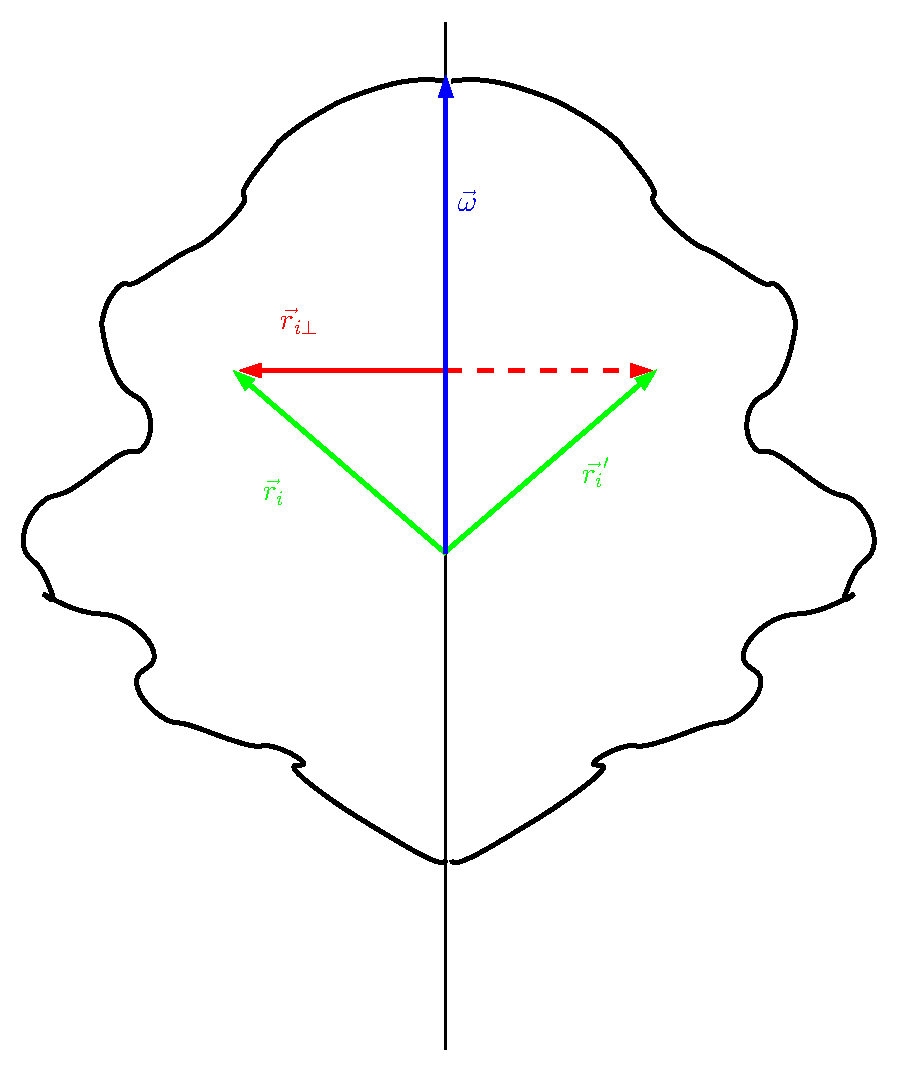
\includegraphics[width=0.5\textwidth]{bilder/rotsym}
   \caption[Drehung: Rotationssymmetrischer Körper]{Ein
     rotationssymmetrischer K"orper wird mit $\vec \omega$ gedreht.}
   \label{abb_rotsym}
\end{figure}




\paragraph{Beispiel: Homogene Kreisscheibe}
\label{kap_beispiel:-homogene-kreisscheibe}

Kreisscheibe der Dicke $D$ und mit dem Radius $R$. Wir arbeiten in
Zylinderkoordinaten: $\diff V = \diff z \cdot r \diff
\varphi \cdot \diff r$. Die (Massen)Dichte ist gleichverteilt: $\varrho =
\varrho_0 = \const$. 

$$
I = \varrho \int_0^R  \int_0^{2\pi} \int_0^D r^2 \diff z \cdot z \diff
\varphi \cdot \diff r = \frac{1}{2}  \underbrace{ \varrho \cdot
\underbrace{\underbrace{\pi
    R^2}_G \cdot D}_V}_M \cdot R^2 = \boxed{I_\text{Zyl} = \frac{1}{2}
M R^2 }
$$



 \paragraph{Beispiel: Hohlzylinder}
 \label{kap_beispiel:-hohlzylinder}


 \textbf{Hohlzylinder:}
Die Wandst"arke sei $d \ll R$. Wir ersetzen also das Integral
$\int_0^R\diff r$ gegen $\int_{R - d}^R\diff r$. Es ergibt
sich dann
$$
I =  2 \pi D \varrho \frac{1}{4} \left [ R^4 - (R-d)^4 \right ] = 
\frac{1}{2} \pi D \varrho [
\underline{4\, d\,{R}^{3}}-6\,{d}^{2}\,{R}^{2}+4\,{d}^{3}\,R-{d}^{4} ] \approx 2\pi
D \varrho R^3d
$$
Und f"ur die Masse ergibt sich
$$
M = \varrho \cdot [ \pi R^2 - \pi (R-d)^2 ] \cdot D = \varrho [
\underline{ 2\pi R d} - \pi d^2 ] \cdot D \approx 2 \varrho \pi R d D
$$
Und damit 
\begin{equation}
   \label{eq:48}
   \boxed{
I_\text{Hohlzyl} \approx M \cdot R^2
}
\end{equation}


Dabei haben wir beide Male eine h"aufig verwendete {N"aherung} gemacht
(bei den unterstrichenen Stellen): Da $d \ll R$, haben wir zuerst brav
mit $d$ und $R$ gerechnet, im Anschluss aber alle Terme, die $d$ in
einer h"oheren Potenz ($d^n$ mit $n \geq 2$) enthielten, einfach
weggelassen.

\begin{Wichtig}
   [\index{N"ahren}Technik: N"ahren]
M"ochte man einen sehr kleinen Wert $d$ ann"ahren, so l"asst man f"ur die
$n$-te N"aherung alle Summanden weg, die $d^m$ mit $m > n$ enthalten.

Bei Polynomen ist dies einfach, bei einer Funktion muss man diese
zuerst \textsc{Taylor}-entwickeln.
\end{Wichtig}

Alternativ h"atten wir die Rechnung auch mithilfe der
\emph{\index{Delta-Distribution}Delta-Distribution} machen k"onnen.
\begin{Beispiel}
   Dazu bestimmen wir die (homogene) "`Oberfl"achendichte"' $\sigma$
   mit $\sigma = \frac{M_0}{2\pi R L}$. Unser Integral vereinfacht
   sich dann zu ($r^2$ ist aus (\ref{eqn_I_rotsym}) und das weitere
   $r$ der Jacobian)
   \begin{equation*}
      I = \int_0^{2\pi} \int_0^L  \int_0^R \sigma r^3 \cdot \delta(R - r)
       \, \diff r \diff z
      \diff \varphi
   \end{equation*}
Das Argument der Delta-Distribution verschwindet bei $r = R$, damit
folgt f"ur das Integral
\begin{equation*}
   I = 2\pi \cdot L \cdot \sigma \, R^3 = 
2\pi \cdot L \cdot \frac{M_0}{2\pi R L} R^3 = 
M_0R^2
\end{equation*}
\end{Beispiel}




\subsubsection{Rotationssymmetrische K"orper, die nicht um K"orperachse Rotieren:
Satz von \textsc{Steiner}}
\label{kap_rotationssymmetrische-korper-nicht-um-korperachse}

Wenn die Rotationsachse \emph{parallel} zur K"orperachse verl"auft,
berechnen wir $I_S$ f"ur die K"orperachse (also die Achse, bez"uglich der
der K"orper symmetrisch ist). Dann gilt
\begin{Wichtig}
   [\index{Satz von \textsc{Steiner}}Satz von \textsc{Steiner}]
   \begin{equation}
      \label{eqn_satz_steiner}
      \boxed{ I = M \cdot a^2 + I_S }
   \end{equation}
mit Drehmoment $I_S$ auf der K"orperachse und Abstand $a$ zwischen
Rotations- und K"orperachse.
\end{Wichtig}













\subsection{Kreisbewegung III -- Der eiernde Kreisel}
\label{kap_kreisbewegung-iii-kreisel}


Wir betrachten einen starren, rotationssymmetrischen K"orper mit $\vec
L \| \vec \omega$ wobei keine "au"seren Drehmomente angreifen -- also
ist $\vec M = 0$ \Impl $\frac{\diff }{\diff t} \vec L = 0$ \Impl $\vec
L = \const$. Der Kreisel kreiselt also brav um seine Figurenachse...


Nun lassen wir eine Kraft $\vec F$ an der Kreiselachse angreifen --
und damit auch ein Drehmoment $\vec M = \vec r \times \vec F$ und
wollen damit den neuen Dreh\emph{impuls} des Systems bestimmen.

Wegen $\vec M = \dot{\vec L}$ k"onnen wir "uber die Zeit
aufintegrieren\footnote{Interessanterweise k"onnen wir an $\vec M =
  \dot{\vec L}$ auch sehen, dass $\vec M \| \diff \vec L$ sein muss.} und erhalten:
\begin{equation}
   \label{eq:49}
   \int_a^e \vec M \diff t = \int_a^e \dot{\vec L} \diff t = \vec L_e
   - \vec L_a = \Delta \vec L
\end{equation}
D.h. f"ur den resultierenden Drehimpuls $\vec L_e$ erhalten wir
\begin{equation}
   \label{eq:50}
   \vec L_e = \vec L_a + \int_a^e \vec M \diff t
\end{equation}
Da $\vec M \bot \vec L_a$ war, wird $\vec L_e$ \emph{nicht} parallel
zu $\vec L_a$ sein. Der Drehimpuls hat also seine Richtung
ge"andert. Wir zerlegen ihn in $\vec L_\|$ und $\vec L_\bot$ parallel
bzw. senkrecht zur Figurenachse.

"Uber den Zusammenhang $\vec L_i = I_i \cdot \vec \omega_i$ aus
\eqref{eq:44} wobei f"ur verschiedene Rotationsachsen in diesem Falle
$I_i \neq I_j$ -- also $I_\| \neq I_\bot$ -- gilt, ergibt sich so:
\begin{eqnarray}
\nonumber
   \vec L &=& \Ten I \cdot \vec \omega \\
\nonumber
   \vec L_\bot + \vec L_\| &=& I_\bot \cdot \vec \omega_\bot + I_\|
   \cdot \vec \omega_\| \\
   \vec L &\not \parallel & \vec \omega
   \label{eq:51}
\end{eqnarray}
Im Kap. \ref{kap_freie-achsen} haben wir gesehen, dass ein K"orper so
\emph{eiert}. Im speziellen, vorliegenden Fall, wird die Figurenachse
dabei auf einer Kegelfl"ache rotieren.



\begin{figure}[h]
   \centering
   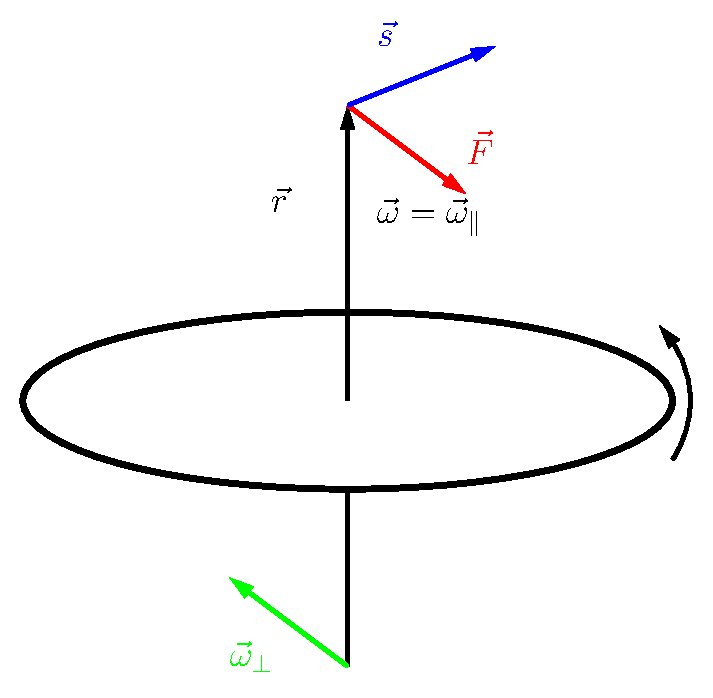
\includegraphics[width=0.7\textwidth]{bilder/kreiselsoerung}
   \caption[Gestörter Kreisel]{Der Kreisel wird mit der Kraft $\vec F$
     gest"ort.}
   \label{abb_kreiselstoerung}
\end{figure}

\bigskip


Wir betrachten jetzt einen \textbf{au"serhalb des Schwerpunkts
  aufgeh"angten Kreisel}: Der Kreisel kreiselt um seine K"orperachse und
deren Verl"angerung ist im Abstand $R$ (mit Vektor $\vec R$) vom
Schwerpunkt entfernt aufgeh"angt.

Es wirkt also die Schwerkraft $\vec F_g$ nach \emph{unten} und dadurch
wirkt auf den Kreis ein Drehmoment $\vec M = \vec R \times \vec F_g$
wodurch $\vec L = \vec L (t) \neq \const$ gilt. In
Abb. \ref{abb_kreisel_aeussere-aufhaengung} w"urde sich die Spitze von
$\vec R$ deswegen \emph{senkrecht} zur Papierebene bewegen -- wie in
Abb. \ref{abb_kreisel_vektoren} versuchsweise angedeutet ist.


Wegen $\vec M = \frac{\diff \vec L}{\diff t }$ gilt $\diff \vec L \|
\vec M$ und aus dem geometrischen Zusammenhang gilt $\|\diff \vec L \|=
\|\vec L \|\cdot \diff \phi$ so gilt auch
\begin{equation}
   \label{eq:52}
   \|\diff \vec L\| = \|\vec L\| \cdot \diff \phi = \|\vec M\| \cdot
   \diff t \text{ bzw. } \diff L = L \diff \phi = M \diff t
\end{equation}
Und der Vektor $\vec R$ w"urde sich mit einer Winkelgeschwindigkeit von 
\begin{equation}
   \label{eq:53}
   \omega_p = \frac{\diff \phi}{\diff t} = \frac{M}{L} = \frac{M}{I
     \cdot \omega} ~ \Rightarrow ~ \omega_p \sim \frac{1}{L} \sim \frac{1}{\omega}
\end{equation}
bewegen. Diese Bewegung nennt man
\textbf{\index{Pr"azession}Pr"azession}. Dabei ist $\omega$ die
Winkelgeschwindigkeit, mit der der Kreisel selbst um seine
K"orperachse rotiert und $\omega_p$ die \emph{Pr"azessionsfrequenz}.
 
\bigskip

Wenn der Kreisel nun anfangs nicht waagerecht aufgeh"angt war, sondern
der Winkel $\alpha$ zwischen $\vec L$ und $\vec F_g$ lag, so gilt
statt Gl. \eqref{eq:53}:
\begin{equation}
   \label{eq:54}
   \omega_p = \frac{\diff \phi}{\diff t} = \frac{M}{L \, \sin\alpha}
\end{equation}

\begin{figure}
   \centering \subfigure[\label{abb_kreisel_aeussere-aufhaengung}Kreisel mit Aufh"angung
   au"sen]{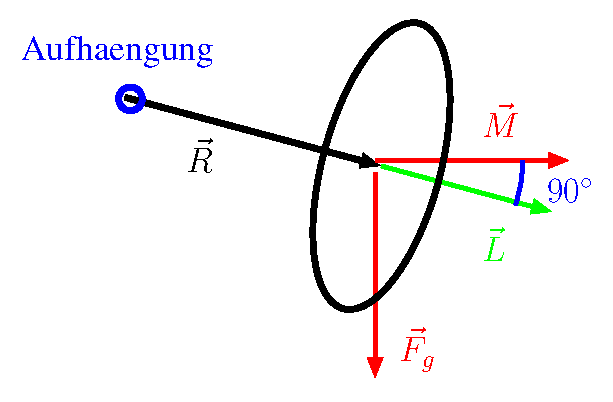
\includegraphics[width=0.5\textwidth]{bilder/praezessionA}}
   \subfigure[\label{abb_kreisel_vektoren}Die Vektoren]{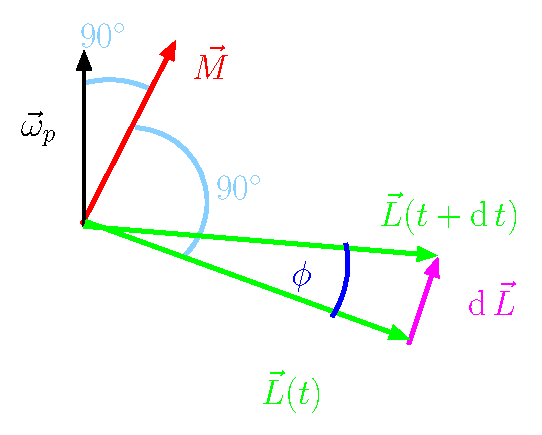
\includegraphics[width=0.4\textwidth]{bilder/praezessionB}}
   \caption{Abbildungen zur Pr"azession}
   \label{abb_preazession}
\end{figure}






\subsection{Ausblick: Quantisierung des Drehimpulses}
\label{kap_ausblick:-quantisierung-des-drehimpulses}

In der Quantenmechanik wird der Drehimpus eine \emph{gequantelte}
Gr"o"se sein -- also nur als (halb oder) ganzzahliges Vielfaches einer
fundamentalen Grundeineit auftreten. Diese Grundeinheit hei"st
\emph{\textsc{\index{Planck'sches Wirkungsquantum}Planck}'sches
  Wirkungsquantum} $\hbar$, also
$$
L = 2 \cdot n \cdot \hbar ~ ~  n \in \mathbb N
$$
wobei 
$$
\hbar = \frac{h}{2\pi} \approx 1,057 \cdot 10^{-34}
\frac{\operatorname{kg\,m^3}}{\operatorname{s}}
$$
Dabei gilt f"ur die Energie
$$
E = \nu \cdot h = \hbar \cdot \omega
$$

So tritt bspw. im hantelf"ormigen $\operatorname{N_2}$-Molek"ul der
Imupls auf als
$$
L = I \cdot \omega = 2mr^2 \cdot \omega = \hbar ~ \Rightarrow ~ \omega
= \frac{\hbar}{2mr^2}
$$
und mit eingesetzten Werten ($2r = 1,11 \operatorname{nm}$, $m = 2,3
\cdot 10^{-26}\operatorname{kg}$) bekommt man
$$
\omega \approx 7,5 \cdot 10^{11} \frac{1}{\operatorname{s}}
$$
und dies entspricht einer Frequenz im \emph{Infrarot}-Bereich.









\section{Vergleich Translation -- Rotation}
\label{kap_vergleich-translation-rotation}

\begin{center}

   \begin{tabular}{l c  l c}
      \toprule
      \textbf{Translation} &  \textit{Formel} & \textbf{Rotation} &
      \textit{Formel} \\
      \midrule
      L"ange & $l$, $s$ & Winkel & $\varphi$ \\
      Masse & $m$ & Tr"agheitsmoment & $\Ten I$ \\
      Geschwindigkeit & $\dot{\vec r} = \vec v$ &
      Winkelgeschwindigkeit & $\dot{\vec \varphi} = \vec \omega$ \\
      Impuls & $\vec p = m \cdot \vec v$ & Drehimpuls & $\vec L = \vec r
      \times \vec p = \Ten I \cdot \vec \omega$ \\
      Kraft & $\vec F = \frac{\diff \vec p}{\diff t }$ & Drehmoment & $\vec M =
      \frac{\diff \vec L}{\diff t}$ \\
      Kinetische Energie & $E_{kin} = \frac{1}{2}mv^2$ & Kinetische Energie
      & $E_{kin} = \frac{1}{2} I \vec \omega^2 = \frac{1}{2} \vec{\omega}^T \Ten I \vec \omega$ \\
      R"uckstellkraft & $\vec F = -D \cdot \vec r$ & R"uckstelldrehmoment &
      $\vec M = -D \cdot \vec \varphi$ \\
      \bottomrule
   \end{tabular}
\end{center}
























%%%%%%%%%%%%%%%%%%%%%%%%%%%%%%%%%%%%%%%%%%%%%%%%%%%%%%%%%

%%%%%%%%%%%%%%%%%%%%%%%%%%%%%%%%%%%%%%%%%%%%%%%%%%%%%%%%%

%%%%%%%%%%%%%%%%%%%%%%%%%%%%%%%%%%%%%%%%%%%%%%%%%%%%%%%%%


